\documentclass[tikz,border=10pt]{standalone}
\usepackage{tikz}
\usetikzlibrary{arrows.meta,positioning,shapes.geometric,fit,backgrounds,calc}
\usepackage{amsmath,amssymb}

\begin{document}

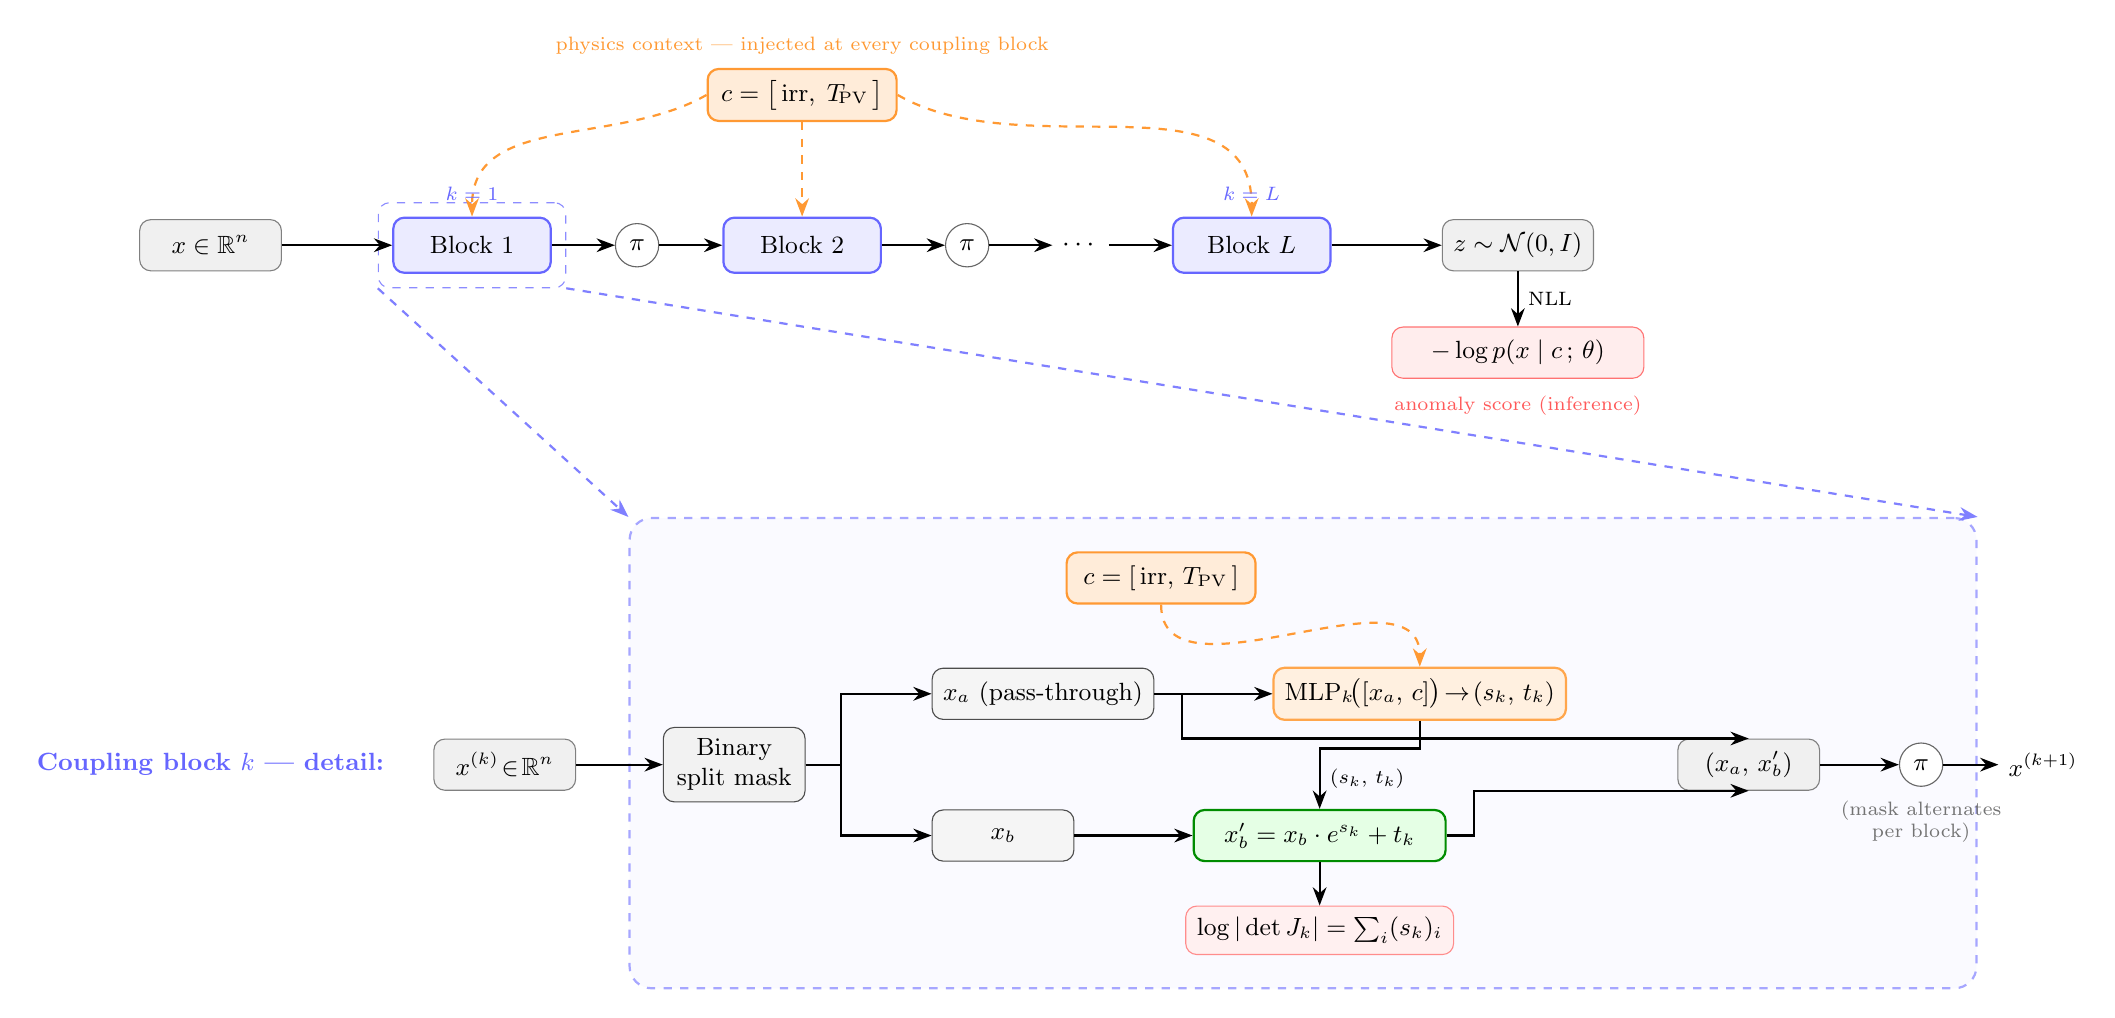
\begin{tikzpicture}[
    every node/.style={font=\small},
    box/.style={
        rectangle, draw=black!70, rounded corners=4pt,
        minimum width=1.8cm, minimum height=0.65cm,
        align=center, inner sep=4pt},
    cblock/.style={
        rectangle, draw=blue!60, thick, rounded corners=4pt,
        fill=blue!8, minimum width=2.0cm, minimum height=0.7cm,
        align=center, inner sep=4pt},
    ctxbox/.style={
        rectangle, draw=orange!80, thick, rounded corners=4pt,
        fill=orange!15, minimum width=2.4cm, minimum height=0.65cm,
        align=center, inner sep=4pt},
    iobox/.style={
        rectangle, draw=black!50, rounded corners=4pt,
        fill=gray!12, minimum width=1.8cm, minimum height=0.65cm,
        align=center, inner sep=4pt},
    scorebox/.style={
        rectangle, draw=red!55, rounded corners=4pt,
        fill=red!7, minimum width=3.2cm, minimum height=0.65cm,
        align=center, inner sep=4pt},
    mlpbox/.style={
        rectangle, draw=orange!70, thick, rounded corners=4pt,
        fill=orange!12, minimum width=3.2cm, minimum height=0.65cm,
        align=center, inner sep=4pt},
    transbox/.style={
        rectangle, draw=green!55!black, thick, rounded corners=4pt,
        fill=green!10, minimum width=3.2cm, minimum height=0.65cm,
        align=center, inner sep=4pt},
    logdetbox/.style={
        rectangle, draw=red!45, rounded corners=4pt,
        fill=red!6, minimum width=3.2cm, minimum height=0.6cm,
        align=center, inner sep=4pt},
    permcirc/.style={
        circle, draw=black!60, fill=white,
        minimum size=0.55cm, inner sep=1pt},
    arr/.style={->, >=Stealth, thick},
    darr/.style={->, >=Stealth, thick, dashed, draw=orange!80},
    zarr/.style={->, >=Stealth, thick, dashed, draw=blue!50},
]

%% ─────────────────────────────────────────────────────────────────────────
%% ROW 1: Overall pipeline
%% ─────────────────────────────────────────────────────────────────────────

\node[iobox] (x_in) {$x \in \mathbb{R}^n$};

\node[cblock, right=1.4cm of x_in]  (B1) {Block $1$};
\node[permcirc, right=0.8cm of B1]  (pi1) {$\pi$};
\node[cblock, right=0.8cm of pi1]   (B2) {Block $2$};
\node[permcirc, right=0.8cm of B2]  (pi2) {$\pi$};
\node[right=0.8cm of pi2, font=\normalsize] (dots) {$\cdots$};
\node[cblock, right=0.8cm of dots]  (BL) {Block $L$};
\node[iobox, right=1.4cm of BL]     (z_out) {$z\sim\mathcal{N}(0,I)$};

\draw[arr] (x_in) -- (B1);
\draw[arr] (B1) -- (pi1);
\draw[arr] (pi1) -- (B2);
\draw[arr] (B2) -- (pi2);
\draw[arr] (pi2) -- (dots);
\draw[arr] (dots) -- (BL);
\draw[arr] (BL) -- (z_out);

% Score node: inference output, far right
\node[scorebox, below=0.7cm of z_out] (score)
    {$-\log p(x\mid c\,;\,\theta)$};
\draw[arr] (z_out) -- node[right, font=\scriptsize] {NLL} (score);
\node[font=\scriptsize, text=red!65, below=0.1cm of score, align=center]
    {anomaly score (inference)};

% Physics context box — prominent, centred above the pipeline
\node[ctxbox, above=1.2cm of B2] (ctx)
    {$c=\bigl[\,\text{irr},\;T_{\!\text{PV}}\,\bigr]$};
\node[font=\scriptsize, text=orange!80, above=0.05cm of ctx]
    {physics context — injected at every coupling block};

\draw[darr] (ctx.west) to[out=210,in=90] (B1.north);
\draw[darr] (ctx)                         -- (B2.north);
\draw[darr] (ctx.east) to[out=-30,in=90] (BL.north);

% Block-index annotations
\node[above=0.08cm of B1, font=\scriptsize, text=blue!60] {$k=1$};
\node[above=0.08cm of BL, font=\scriptsize, text=blue!60] {$k=L$};

%% ─────────────────────────────────────────────────────────────────────────
%% ROW 2: Coupling block detail  (6cm below top row)
%% ─────────────────────────────────────────────────────────────────────────

\node[font=\small\bfseries, text=blue!60,
      below=6.0cm of x_in] (zoom_label) {Coupling block $k$ — detail:};

% Input
\node[iobox, right=0.5cm of zoom_label] (x_in2) {$x^{(k)}\!\in\!\mathbb{R}^n$};

% Binary split
\node[box, fill=gray!10, right=1.1cm of x_in2] (split) {Binary\\split mask};
\draw[arr] (x_in2) -- (split);

% Upper partition: pass-through
\node[box, fill=gray!8, right=1.6cm of split, yshift= 0.9cm] (xa)
    {$x_a$ \small(pass-through)};
% Lower partition: transformed
\node[box, fill=gray!8, right=1.6cm of split, yshift=-0.9cm] (xb)
    {$x_b$};

\draw[arr] (split.east) -- ++(0.45,0) |- (xa.west);
\draw[arr] (split.east) -- ++(0.45,0) |- (xb.west);

% Physics context input — inside detail panel
\node[ctxbox, above=0.8cm of xa, xshift=1.5cm] (ctx2)
    {$c=[\,\text{irr},\,T_{\text{PV}}\,]$};

% MLP (orange box, same row as xa)
\node[mlpbox, right=1.5cm of xa] (mlp)
    {MLP$_k\!\bigl([x_a,\,c]\bigr)\!\to\!(s_k,\,t_k)$};
\draw[arr] (xa) -- (mlp);
\draw[darr] (ctx2.south) to[out=270,in=90] (mlp.north);

% Transform (green, same row as xb)
\node[transbox, right=1.5cm of xb] (trans)
    {$x_b' = x_b \cdot e^{s_k} + t_k$};
\draw[arr] (xb) -- (trans);

% (s_k, t_k) arrow from MLP south down to transform north
\draw[arr] (mlp.south) -- ++(0,-0.35)
    -| node[near end, right, font=\scriptsize] {$(s_k,\,t_k)$} (trans.north);

% Log-det accumulation
\node[logdetbox, below=0.55cm of trans] (logdet)
    {$\log|\det J_k|=\textstyle\sum_i (s_k)_i$};
\draw[arr] (trans.south) -- (logdet.north);

% Recombine
\node[iobox, right=1.4cm of mlp, yshift=-0.9cm] (out2) {$(x_a,\,x_b')$};
\draw[arr] (xa.east)    -- ++(0.35,0) |- (out2.north);
\draw[arr] (trans.east) -- ++(0.35,0) |- (out2.south);

% Post-block permutation
\node[permcirc, right=1.0cm of out2] (pi3) {$\pi$};
\node[font=\scriptsize, text=black!55, below=0.05cm of pi3, align=center]
    {(mask alternates\\per block)};
\draw[arr] (out2) -- (pi3);
\draw[arr] (pi3.east) -- ++(0.7,0)
    node[right, font=\small] {$x^{(k+1)}$};

%% ─────────────────────────────────────────────────────────────────────────
%% Background: bounding box for detail panel (includes ctx2)
%% ─────────────────────────────────────────────────────────────────────────
\begin{scope}[on background layer]
  \node[draw=blue!35, dashed, thick, rounded corners=8pt,
        fill=blue!2, inner sep=12pt,
        fit=(split)(xa)(xb)(ctx2)(mlp)(trans)(logdet)(out2)(pi3)] (bbox) {};
\end{scope}

%% ─────────────────────────────────────────────────────────────────────────
%% Zoom connector: dashed box around Block 1 → funnel down to detail bbox
%% ─────────────────────────────────────────────────────────────────────────
\begin{scope}[on background layer]
  \node[draw=blue!45, dashed, rounded corners=4pt,
        inner sep=5pt, fit=(B1)] (zoombox) {};
  \draw[zarr] (zoombox.south west) -- (bbox.north west);
  \draw[zarr] (zoombox.south east) -- (bbox.north east);
\end{scope}

\end{tikzpicture}
\end{document}
